% (c) 2015 Daniele Zambelli daniele.zambelli@gmail.com
% (c) 2016 Andrea Sellaroli andrea.sellaroli@istruzione.it

\chapter{Variabili aleatorie}

\'E curioso osservare che uno dei settori più rigogliosi e applicati della matematica non sia quello deterministico e ``rigido'' legato ad enunciati e regole ben note, ma quello \emph{stocastico}, regolato da leggi e fenomeni che si verificano con una certa probabilità. Dinamica di popolazioni, previsioni metereologiche, mercati finanziari sono solo alcune delle applicazioni più rigogliose della matematica, tutte fondate sull'analisi stocastica.\\

Per cominciare, facciamo un esempio: un arciere molto bravo scaglia 3 frecce contro un bersaglio. Poiché è molto bravo, ad ogni tentativo ha una buona probabilità di centrare il bersaglio, che supponiamo pari al \(90\%\). Ci chiediamo quale sia la probabilità che centri il bersaglio tutte e 3 le volte, solo 2 volte, 1 volta o nemmeno una.
\[ P(\text{3 centri})= P\tonda{\text{\boxed{X} \, \boxed{X} \, \boxed{X}}} = P \tonda{\text{\boxed{X}}} \cdot P \tonda{\text{\boxed{X}}} \cdot P \tonda{\text{\boxed{X}}} = \dfrac{90}{100} \cdot \dfrac{90}{100}  \cdot \dfrac{90}{100}   = 
72,9\%. \]
dove abbiamo usato la formula per l'evento intersezione, sfruttando il fatto che possiamo supporre indipendenti gli eventi `'Centrare il primo bersaglio'', ``Centrare il secondo bersaglio'' e ``Centrare il terzo bersaglio'' (per essere pignoli, il secondo tentativo potrebbe essere influenzato dal primo: se ho sbagliato, mi agito e tiro peggio, oppure potrei concentrarmi meglio). Calcoliamo gli altri 3 casi in modo simile:
\[ \begin{split} P(\text{2 centri})&= P\tonda{\text{\boxed{X} \, \boxed{X} \, \boxed{O}} \text{ oppure } \text{\boxed{X} \, \boxed{O} \, \boxed{X}} \text{ oppure } \text{\boxed{O} \, \boxed{X} \, \boxed{X}}} =\\ &= 
P\tonda{\text{\boxed{X} \, \boxed{X} \, \boxed{O}}} +P\tonda{\text{\boxed{X} \, \boxed{O} \, \boxed{X}}} + P\tonda{ \text{\boxed{O} \, \boxed{X} \, \boxed{X}}} =\\ &=
 \tonda{\dfrac{90}{100} \cdot \dfrac{90}{100}  \cdot \dfrac{10}{100}}+ \tonda{\dfrac{90}{100} \cdot \dfrac{10}{100}  \cdot \dfrac{90}{100}}+ \tonda{\dfrac{10}{100} \cdot \dfrac{90}{100}  \cdot \dfrac{90}{100} }  = 24,3 \%  \end{split}\]
 
 ricordando la formula per la probabilità dell'evento unione ed osservando che i 3 eventi sono incompatibili. Proseguendo in modo simile:
 \[ \begin{split} P(\text{1 centro})&= P\tonda{\text{\boxed{X} \, \boxed{O} \, \boxed{O}} \text{ oppure } \text{\boxed{O} \, \boxed{X} \, \boxed{O}} \text{ oppure } \text{\boxed{O} \, \boxed{O} \, \boxed{X}}} =\\ &= 
P\tonda{\text{\boxed{X} \, \boxed{O} \, \boxed{O}}} +P\tonda{\text{\boxed{O} \, \boxed{X} \, \boxed{O}}} + P\tonda{ \text{\boxed{O} \, \boxed{O} \, \boxed{X}}} =\\ &=
 \tonda{\dfrac{90}{100} \cdot \dfrac{10}{100}  \cdot \dfrac{10}{100}}+ \tonda{\dfrac{10}{100} \cdot \dfrac{90}{100}  \cdot \dfrac{10}{100}}+ \tonda{\dfrac{10}{100} \cdot \dfrac{10}{100}  \cdot \dfrac{90}{100} } = 2,7 \%  \end{split}\]
 e infine l'ultimo caso, come il primo:
\[ P(\text{0 centri})= P\tonda{\text{\boxed{O} \, \boxed{O} \, \boxed{O}}} = P \tonda{\text{\boxed{O}}} \cdot P \tonda{\text{\boxed{O}}} \cdot P \tonda{\text{\boxed{O}}} = \dfrac{10}{100} \cdot \dfrac{10}{100}  \cdot \dfrac{10}{100}   = 
0,1\%. \]
Quello che abbiamo appena costruito è una variabile aleatoria discreta \(X = \{\text{numero di centri}\}\) che può assumere 4 valori diversi \(\{0,1,2,3\}\) ciascuno con una propria probabilità.

\section{Variabili aleatorie discrete}
\label{sec:01_discrete}

Studiamo un \emph{esperimento aleatorio}, ovvero un esperimento che può avere vari esiti possibili, ciascuno con una sua probabilità, e uno \emph{spazio degli eventi elementari} $\Omega$, ovvero l'insieme di tutti i diversi esiti che può avere l'esperimento.

\begin{definizione} Chiamiamo \emph{variabile aleatoria discreta} una variabile che può assumere valori discreti $\{x_1,x_2\dots,x_n\}$ a seconda del verificarsi o meno degli eventi $\{E_1, E_2,\dots, E_n\}$, tra loro incompatibili e tali che $E_1 \cup E_2 \cup \dots \cup E_n = \Omega$.
\end{definizione}

Entrando nel dettaglio, si potrebbe dire che una variabile aleatoria X è una funzione che associa ad ogni evento un valore discreto, cioé $X:\Omega \longrightarrow \mathbb{R}\,, E \longmapsto X(E)$. La condizione di incompatibilità e completamento di $\Omega$ è una cosa tecnica che serve a far si che questa funzione sia sempre ``funzionante'', ovvero restituisca \underline{\smash{sempre}} un \underline{unico} valore.
\begin{osservazione} I valori discreti che la variabile X può assumere non sono necessariamente un numero finito $\{x_1,x_2\dots,x_n\}$. Si possono estendere in modo semplice tutte le definizioni al caso infinito (numerabile) sostituendo somme con serie, con qualche piccolo accorgimento.
\end{osservazione}

\begin{esempio} Lancio un dado a 6 facce. Variabile aleatoria $X=\{\text{numero uscito}\}$\\[3pt]
Gli eventi sono $E_1 = $\{esce 1\}, $E_2 = $\{esce 2\}, \dots, $E_6 = $\{esce 6\} ed è chiaro che gli eventi sono tutti incompatibili tra loro (non può uscire, con lo stesso tiro di dadi, sia 1 che 3) e l'unione di tutti questi eventi dà l'intero spazio degli eventi (infatti può uscire solo un numero tra 1 e 6). \\I valori che può assumere questa variabile sono $x_1=1, x_2=2, \dots, x_6=6$.
\end{esempio}

Ad ogni valore, che può essere assunto dalla variabile X, possiamo associare la probabilità che X assuma veramente tale valore. Definiamo perciò:
\[\boxed{p_i = P(X=x_i)} \qquad \longrightarrow \qquad \text{probabilità che X assuma il valore $x_i$}\]
Possiamo notare subito che valgono le proprietà: \qquad\(\boxed{p_i \in [0,1]} \quad \boxed{p_1+p_2+\dots+p_n=1}\) 

\begin{definizione}Chiamiamo \emph{distribuzione di probabilità} della variabile aleatoria X la successione delle probabilità $p_1,p_2,\dots,p_n$ associate ai valori $x_1,x_2,\dots,x_n$ che la variabile X può assumere. 
\end{definizione}

\'E solitamente una buona abitudine sintetizzare tale distribuzione in una tabella, maggiormente leggibile:
\[x_1=1,\, x_2=4,\, x_3 = 7 \qquad p_1=\dfrac{2}{7},\, p_2 = \dfrac{4}{7},\, p_3 = \dfrac{1}{7} \qquad \longrightarrow \quad 
\renewcommand\arraystretch{1.4}
\setlength\arraycolsep{25pt}
\begin{tabular}{c|c|c|c}
$X$ & 1 & 4 & 7\\
\hline
$p$ & 2/7 & 4/7 & 1/7\\
\end{tabular}\]
\'E possibile inoltre rappresentare la distribuzione di probabilità con un \emph{istogramma} o un \emph{diagramma cartesiano}.

\begin{figure}[htpb!]
  \centering
  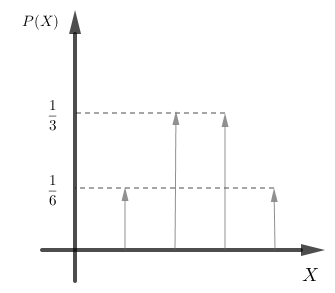
\includegraphics[width=0.45\textwidth]{img/diagramma.png}
  \includegraphics[width=0.45\textwidth]{img/istogramma.png}
  \caption{Diagramma cartesiano e istogramma}
  %\label{fig:1_2}
\end{figure}

\begin{esempio} Lancio 3 volte una moneta. Variabile aleatoria $X = \{\text{numero di ``testa'' usciti}\}$:
\[\begin{split}p_1 &= P(X=0) = P(\text{\boxed{CCC}}) = \tonda{\dfrac{1}{2}}^3 = 0,125 \\
p_2 &= P(X=1) = P(\text{\boxed{TCC}}\, o\, \text{\boxed{CTC}} \, o\, \text{\boxed{CCT}}) = \tonda{\dfrac{1}{2}}^3 + \tonda{\dfrac{1}{2}}^3 + \tonda{\dfrac{1}{2}}^3= 3\cdot \tonda{\dfrac{1}{2}}^3 = 0,375 \\
p_3 &= P(X=2) = P(\text{\boxed{TTC}} \, o\, \text{\boxed{CTT}}\, o\, \text{\boxed{TCT}}) = \tonda{\dfrac{1}{2}}^3 + \tonda{\dfrac{1}{2}}^3 + \tonda{\dfrac{1}{2}}^3= 3 \cdot \tonda{\dfrac{1}{2}}^3 = 0,375 \\
p_4 &= P(X=3) = P(\text{\boxed{CCC}}) = \tonda{\dfrac{1}{2}}^3 = 0,125 \\
 \end{split}\]
 Possiamo quindi scrivere la distribuzione di X come: \quad \(\renewcommand\arraystretch{1.4}
\setlength\arraycolsep{25pt}
\begin{tabular}{c|c|c|c|c}
$X$ & 0 & 1 & 2 & 3\\
\hline
$p$ & 0,125 & 0,375 & 0,375 & 0,125\\
\end{tabular}\)
\end{esempio}

\begin{definizione}
La \emph{funzione di ripartizione} della variabile $X$ è la funzione $F: \mathbb{R} \longmapsto [0,1]$ che associa ad ogni valore reale la probabilità che X assuma valori non superiori a quello dato, ovvero $F(x) := P(X\leq x)$
\end{definizione}

Per le variabili discrete, la funzione di ripartizione non è continua, e in particolare:
\[\lim_{x \rightarrow +\infty} F(x) = 1 \qquad \lim_{x \rightarrow -\infty} F(x) = 0 \hspace{1.5cm} F(x_i) = p_1+p_2+\dots+p_i  \qquad \forall i=1,\dots,n\]

\begin{esempio} Lancio 3 volte un dado. Variabile aleatoria $X = \{ \text{numero di dadi con valore pari}\}$\\

\begin{minipage}[c]{.45\textwidth}
\renewcommand\arraystretch{1.4}
\setlength\arraycolsep{25pt}
 \quad \begin{tabular}{c|c|c|c|c}
$X$ & 0 & 1 & 2 & 3\\
\hline
$p$ & 1/8 & 3/8 & 3/8 & 1/8\\
\hline
$F(X)$ & 1/8 & 4/8 & 7/8 & 1\\
\end{tabular}
\end{minipage}\hfil
\begin{minipage}[c]{.55\textwidth}
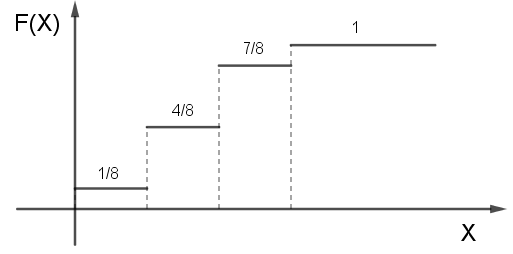
\includegraphics[width=0.8\textwidth]{img/ripartizione.png}
\end{minipage}
\end{esempio}

\subsection{Valori sintetici delle distribuzioni}

Come per l'analisi statistica, anche per le variabili aleatorie è possibile racchiudere buona parte dell'informazionerelativa alla distribuzione in 2 soli valori: il valor medio e la varianza.\\
Il valor medio, detto anche \emph{speranza matematica} (o valore atteso), ci dà un'indicazione teorica del valore centrale intorno a cui si distribuiscono i valori rilevati dalla variabile X. 
\[\text{\textbf{Valor medio ($\mu$)}:} \quad M(X) = x_1 \cdot p_1+\dots + x_n \cdot p_n  \quad \rightarrow \quad \boxed{M(X) = \sum_{i = 1}^n x_i \cdot p_i}\]
La varianza ci permette invece di dare una stima della concentrazione dei valori vicino al valor medio. Più la varianza è piccola e più la distribuzione della variabile X si concentra vicino alla media $\mu$.
\[\text{\textbf{Varianza ($\sigma^2$)}:} \quad V(X) = (x_1-\mu)^2 \cdot p_1+\dots + (x_n-\mu)^2 \cdot p_n  \quad \rightarrow \quad \boxed{V(X) = \sum_{i = 1}^n (x_i-M(X))^2 \cdot p_i}\]
\begin{esempio} Riprendiamo la distribuzione vista in precedenza:\\[4pt]

\begin{minipage}[r]{.4\textwidth}
\renewcommand\arraystretch{1.4}
\setlength\arraycolsep{25pt}
 \quad \begin{tabular}{c|c|c|c|c}
$X$ & 0 & 1 & 2 & 3\\
\hline
$p$ & 1/8 & 3/8 & 3/8 & 1/8
\end{tabular}
\end{minipage}\hfil
\begin{minipage}[c]{.55\textwidth}
\[ M(X) = 0\cdot \dfrac{1}{8}+1\cdot \dfrac{3}{8}+2\cdot \dfrac{3}{8}+4\cdot \dfrac{1}{8} = \dfrac{13}{8} \approx 1,6\]
\end{minipage}
\[ V(X) = (0-1,6)^2\cdot \dfrac{1}{8}+(1-1,6)^2\cdot \dfrac{3}{8}+(2-1,6)^2\cdot \dfrac{3}{8}+(4-1,6)^2\cdot \dfrac{1}{8} \approx 1,23\]
\end{esempio}

\subsection{Proprietà dei valori sintetici}

 Dimostriamo alcune relazioni e proprietà utili per il calcolo del valor medio e della varianza. Per farlo è necessario prima definire alcune operazioni che è possibile fare con le variabili aleatorie:
 \begin{itemize}
 \item Definiamo $Y = X+a$ la variabile aleatoria che si ottiene sommando il numero $a\in \mathbb{R}$ alla variabile aleatoria X. Si può mostrare in modo semplice che la distribuzione di probabilità di Y ha gli stessi valori $p_i$ di quella di X;
 \item Definiamo $Y = a\cdot X$ la variabile aleatoria che si ottiene moltiplicando la variabile aleatoria X per il numero $a\in \mathbb{R}$. Anche in questo caso la distribuzione di probabilità di Y ha gli stessi valori $p_i$ di quella di X.
 \end{itemize}
 
 \begin{proprieta} (Valor medio) \quad $\boxed{M(aX) = a\, M(X)}  \quad \boxed{M(X+b) = M(X)+b} \quad \forall a,b \in \mathbb{R}$
 \end{proprieta}
 \begin{proof}
\'E sufficiente applicare proprietà basi della somma.\\
 \[\begin{split}M(aX)&= \sum_{i=1}^n \tonda{a \, x_i } p_i = a \underbrace{\sum_{i=1}^n x_i p_i}_{M(X)} = a \, M(X) \\ 
 M(X+b) &= \sum_{i=1}^n \tonda{x_i+b} p_i = \sum_{i=1}^n \tonda{x_i p_i+b p_i} = \underbrace{\sum_{i=1}^n x_i p_i}_{M(X)} +b  \underbrace{\sum_{i=1}^n p_i}_{1} = M(X)+b\end{split}\]
 \end{proof}
 
  \begin{proprieta} (Varianza) \quad $\boxed{V(aX) = a^2 V(X)} \quad \boxed{V(X+b) = V(X)} \quad \forall a,b \in \mathbb{R}$
 \end{proprieta}
 \begin{proof}
 Usiamo proprietà basi della somma e qualche piccolo accorgimento.\\
 \[\begin{split}V(aX)&= \sum_{i=1}^n \tonda{a \,x_i-M(a\,X)}^2 p_i = \sum_{i=1}^n \tonda{a\,x_i-a\,M(X)}^2 p_i =\\&=  \sum_{i=1}^n [a (x_i-\,\underbrace{M(X)}_{\mu})]^2 p_i =\sum_{i=1}^n a^2 \tonda{x_i-\mu}^2 = a^2 \underbrace{\sum_{i=1}^n \tonda{x_i-\mu}^2 p_i }_{V(X)}= a^2 \cdot V(X) \\
 V(X+b) &= \sum_{i=1}^n \tonda{x_i+b-M(X+b)}^2 p_i = \sum_{i=1}^n \tonda{x_i+\cancel{b}-M(X)-\cancel{b}}^2 p_i = \\ &=\sum_{i=1}^n \tonda{x_i-\mu}^2 p_i = V(X) \end{split}\]
 \end{proof}
 
   \begin{proprieta} (Formula alternativa varianza) \quad $V(X) = M(X^2)-M(X)^2$
 \end{proprieta}
 \begin{proof}
  \[\begin{split} V(X) &= \sum_{i=1}^n \tonda{x_i-\mu}^2 p_i = \sum_{i=1}^n \tonda{x_i^2+\mu^2-2x_i \mu} p_i =\sum_{i=1}^n \tonda{x_i^2 p_i + \mu^2 p_i - 2 \mu x_i p_i}=\\ &= \underbrace{\sum_{i=1}^n x_i^2 p_i}_{M(X^2)} + \sum_{i=1}^n \mu^2 p_i - 2 \sum_{i=1}^n \mu x_i p_i = M(X^2)+\mu^2 \underbrace{\sum_{i=1}^n p_i}_{1}-2 \mu \underbrace{\sum_{i=1}^n x_i p_i}_{\mu}=\\&=
  M(X^2)+\mu^2-2\mu^2 = M(X^2)-\mu^2 = M(X^2)-M(X)^2 \end{split}\]
 \end{proof}
 
 \section{Variabili aleatorie standardizzate}
 \label{sec:02_standardizzate}
 
 \'E spesso utile, per motivi che verranno approfonditi in seguito, standardizzare una variabile aleatoria, ovvero riscalare i suoi valori per ottenere una nuova variabile aleatoria con media nulla e varianza unitaria
 
 \begin{definizione} Data una variabile aleatoria X con media $\mu$ e varianza $\sigma^2$, definiamo la \emph{variabile aleatoria normalizzata} relativa ad X come $\boxed{Z = \dfrac{X-\mu}{\sigma}}$
 \end{definizione}
 
 Ogni variabile aleatoria discreta può essere normalizzata, se ha media e varianza finite.

\begin{proprieta} (Variabile normalizzata) \quad \boxed{M(Z)=0} \quad \boxed{V(Z) = 1}
\end{proprieta}
\begin{proof} \'E solo questione di applicare le proprietà di media e varianza:
\[\begin{split}M(Z) &= M\tonda{\dfrac{X-\mu}{\sigma}} = M\tonda{\dfrac{1}{\sigma} \tonda{X-\mu}} = \dfrac{1}{\sigma} M(X-\mu) = \dfrac{1}{\sigma} (\underbrace{M(X)}_{\mu}-\mu) =  \dfrac{1}{\sigma} (\mu-\mu)=0  \\
V(Z) &= V\tonda{\dfrac{X-\mu}{\sigma}} = V\tonda{\dfrac{1}{\sigma} \tonda{X-\mu}} = \dfrac{1}{\sigma^2} V(X-\mu)=\dfrac{1}{\sigma^2} \underbrace{V(X)}_{\sigma^2} = \dfrac{\sigma^2}{\sigma^2} = 1\end{split}\]
\end{proof}
\section{Distribuzioni discrete di uso comune}
\label{sec:02_distrib_discrete}

\subsection{Distribuzione uniforme}
Pensiamo al lancio di un dado a 6 facce, con variabile aleatoria $X = \{valore ottenuto\}$. Si tratta di una variabile aleatoria discreta (infatti i possibili valori sono i numeri naturali da 1 a 6) e, in particolare, ogni valore ha la stessa probabilità di uscita (a meno di dadi truccati).

\begin{definizione} Chiamiamo \emph{distribuzione discreta uniforme} $\mathcal{U}(n)$ di parametro $n$ la distribuzione di probabilità con uguali valori di ``$p$'', ovvero $p_1=p_2=\dots=p_n$
\end{definizione}
\begin{esempio} Riprendendo il tiro del dado a 6 facce, abbiamo:\\[4pt]
\begin{minipage}[c]{.6\textwidth}
\begin{center}
 \(\renewcommand\arraystretch{1.4}
\setlength\arraycolsep{22pt}
\begin{tabular}{c|c|c|c|c|c|c}
$X$ & 1 & 2 & 3 & 4& 5 &6\\
\hline
$p$ &1/6 & 1/6 &1/6 & 1/6 &1/6 & 1/6 \\
\end{tabular}\)
\end{center}

\end{minipage}
\begin{minipage}[c]{.4\textwidth}
\begin{center}
  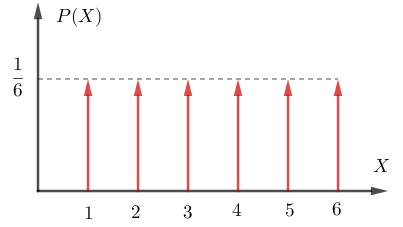
\includegraphics[width=0.95\textwidth]{img/Uniforme_discr.png}
\end{center}
\end{minipage}
\[ \begin{split} M(X) &= 1 \cdot \dfrac{1}{6}+2 \cdot \dfrac{1}{6}+3 \cdot \dfrac{1}{6}+4 \cdot \dfrac{1}{6}+5 \cdot \dfrac{1}{6}+6 \cdot \dfrac{1}{6} = 3,5\\
V(X) &= (1-3,5)^2 \cdot \dfrac{1}{6}+(2-3,5)^2 \cdot \dfrac{1}{6}+\dots+(6-3,5)^2 \cdot \dfrac{1}{6} = \dfrac{35}{12} \approx 2,92  \end{split}\]

\begin{proprieta} Data una variabile discreta uniforme di parametro $n$, si dimostra che: 
\[\boxed{p_i = \dfrac{1}{n} \quad \forall i=1,\dots,n} \qquad \boxed{M(X) = \dfrac{n+1}{2}} \qquad \boxed{V(X) = \dfrac{n^2-1}{12}}\]
\end{proprieta}

\begin{esercizio} Lancio un dado a 30 facce. Variabile aleatoria $X=\{\text{valore ottenuto}\}$. Calcolare media e varianza della distribuzione di X.\\[6pt]
\begin{minipage}[c]{.6\textwidth}
\begin{center}
 \(\renewcommand\arraystretch{1.4}
\setlength\arraycolsep{22pt}
\begin{tabular}{c|c|c|c|c|c|c}
$X$ & 1 & 2 & 3 &  \dots &29&30\\
\hline
$p$ &1/30 & 1/30 & 1/30 &\dots & 1/30& 1/30 \\
\end{tabular}\)
\end{center}

\end{minipage}
\begin{minipage}[c]{.4\textwidth}
\[\begin{split} &M(X) = \dfrac{30+1}{2} = \dfrac{31}{2}=15,5 \\
 &V(X)= \dfrac{30^2-1}{12} = \dfrac{899}{12}=74,9
\end{split}\]
\end{minipage}
\end{esercizio}


\end{esempio}
\subsection{Distribuzione binomiale}

Ritorniamo per un attimo all'esempio iniziale dell'arciere e cerchiamo di ricavare una nuova variabile aleatoria generica, valida anche per quel caso. Possiamo riferirci a quella situazione parlando di \textbf{schema delle prove ripetute} in cui, su un numero totale di prove effettuate (in quel caso, tre), si cerca di studiare il numero di tentativi ``andati a segno''. Il concetto di ``segnare'' può essere esteso in modo banale, parlando di \textbf{successo/insuccesso} (in quel caso il successo era dettato dal centrare o meno il bersaglio, ma qualunque ``successo'' può essere interpretato come un ``centrare il bersaglio''). Proviamo quindi a studiare questa situazione e ricavare una regola generale.

\begin{esempio} Giochiamo ai rigori. Numero di tentativi: $n=5$, probabilità di successo: $p = 70\%=0.7$ (il portiere non è un asso, diciamo!), calcoliamo la probabilità di segnare solamente $k=3$ gol su 5.
\[P(\text{3 gol})= P\tonda{\text{\boxed{XXXOO}} \text{ oppure } \text{\boxed{XXOXO}} \text{ oppure } \text{\boxed{XOOXX}} \text{ oppure } \dots \text{ oppure } \dots} = \]
Ci rendiamo subito conto che, per visualizzare tutti i possibili casi in cui facciamo 3 gol su 5, abbiamo bisogno di molto tempo (sarebbe ancora peggio se ci chiedessimo la probabilità di fare 35 gol su 100). In realtà possiamo notare due cose: 
\begin{itemize}
\item Una volta elencati tutti i casi, ognuno di questi risulta incompatibile con ogni altro, quindi è possibile usare in modo efficace la proprietà dell'evento unione, nel caso di eventi incompatibili ($P(A \cup B) = P(A) +P(B)$);
\item Ognuno di questi eventi ha la stessa probabilità, infatti l'ordine con cui avvengono i gol non ha influenza. Infatti, per esempio:
\end{itemize}
\[\begin{split}P\tonda{\text{\boxed{XXXOO}}} &= P\tonda{\text{\boxed{X}}} \cdot P\tonda{\text{\boxed{X}}} \cdot P\tonda{\text{\boxed{X}}} \cdot P\tonda{\text{\boxed{O}}} \cdot P\tonda{\text{\boxed{O}}}=\\ &= \tonda{\dfrac{70}{100}} \cdot  \tonda{\dfrac{70}{100}} \cdot  \tonda{\dfrac{70}{100}} \cdot  \tonda{1-\dfrac{70}{100}} \cdot \tonda{ 1-\dfrac{70}{100}} =\tonda{\dfrac{70}{100}}^3 \tonda{\dfrac{30}{100}}^2 \end{split}\]

\[\begin{split}P\tonda{\text{\boxed{XXOXO}}} &= P\tonda{\text{\boxed{X}}} \cdot P\tonda{\text{\boxed{X}}} \cdot P\tonda{\text{\boxed{O}}}  \cdot P\tonda{\text{\boxed{X}}} \cdot P\tonda{\text{\boxed{O}}}=\\ &= \tonda{\dfrac{70}{100}} \cdot  \tonda{\dfrac{70}{100}} \cdot  \tonda{1-\dfrac{70}{100}}  \cdot  \tonda{\dfrac{70}{100}} \cdot \tonda{ 1-\dfrac{70}{100}} =\tonda{\dfrac{70}{100}}^3 \tonda{\dfrac{30}{100}}^2 \end{split}\]
Quindi, riprendendo dall'uguaglianza iniziata sopra, abbiamo
\[\begin{split}&= P\tonda{\text{\boxed{XXXOO}}}+P\tonda{\text{\boxed{XXOXO}}}+P\tonda{\text{\boxed{XOOXX}}}+ P(\dots)+\dots = \\ &= \tonda{\dfrac{70}{100}}^3 \tonda{\dfrac{30}{100}}^2+\tonda{\dfrac{70}{100}}^3 \tonda{\dfrac{30}{100}}^2+\tonda{\dfrac{70}{100}}^3 \tonda{\dfrac{30}{100}}^2+\dots \end{split}\]
Rimane solo da capire quante volte ripetere questa somma di uguali quantità. Alla domanda in realtà si può rispondere in modo facile usando il \emph{calcolo combinatorio}: quante disposizioni di 5 elementi si possono creare, dove 3 elementi siano uguali ad X e i rimanenti 2 elementi siano uguali ad O ? Rivedendo un pò le formule ci si accorge che non è altro che una combinazione di 5 elementi da cui ne scelgo 3, perciò:
\[P(\text{3 gol}) = \underbrace{ \tonda{\dfrac{70}{100}}^3 \tonda{\dfrac{30}{100}}^2+\tonda{\dfrac{70}{100}}^3 \tonda{\dfrac{30}{100}}^2+ \dots}_{C_{5,3} \,\text{volte}} = C_{5,3} \cdot \tonda{\dfrac{70}{100}}^3 \tonda{\dfrac{30}{100}}^2\]
Rimpiazzando i valori coi relativi parametri: \quad \( \displaystyle P(X=k)= \binom{n}{k} p^k (1-p)^{n-k}\)\end{esempio}


\begin{definizione} Chiamiamo \emph{distribuzione binomiale} $\mathcal{B}(n,p)$ una variabile aleatoria discreta con due parametri $n \in \mathbb{N}$ e $p \in [0,1]$ tale che:
\[ x_k = k \in \{0,1,\dots,n\} \qquad P(X=k)= \binom{n}{k} p^k (1-p)^{n-k}\]
\end{definizione}

La distribuzione binomiale viene usata solitamente per modellare (ovvero creare un modello matematico) una variabile aleatoria che descrive \textbf{prove ripetute indipendenti}, ovvero una serie di $n$ eventi indipendenti in cui la probabilità di successo è pari a $p$. Il concetto di successo, come espresso a inizio capitolo, è un concetto ampio, che si può adattare a molteplici casistiche. Vediamone alcune:
\begin{itemize}
\item gioco dei rigori: 5 rigori, e so di avere una probabilità di segnare un gol del $40\%$ (perché ho notato che, in genere, su 10 tiri, ne faccio giusti 4):
\[n = 5\; \text{(tentativi)} \qquad p = \dfrac{40}{100} \;\text{(probabilità di fare 1 gol)} \qquad \longrightarrow \qquad \mathcal{B}\tonda{5, \dfrac{40}{100}}\]
\item pesco 13 volte una pallina da un cesto che contiene 4 palline d'oro e le restanti di legno, reinserendo ogni volta la pallina nel cesto. Mi interessa pescare quelle dorate:
\[n = 13\; \text{(tentativi)} \qquad p = \dfrac{4}{13} \;\text{(pesco la pallina dorata)} \qquad \longrightarrow \qquad \mathcal{B}\tonda{13, \dfrac{4}{13}}\]
\item scatola di lampadine: ne pesco 7 (ma ogni volta reinserisco anche quella pescata nella scatola). So che il $3\%$ delle lampadine è difettoso. Il successo in questo caso è ``trovare quella difettosa'', semplicemente perché è ciò che mi interessa fare: trovare le difettose!!
\[n = 7\; \text{(tentativi)} \qquad p = \dfrac{3}{100} \;\text{(trovo una lampadina difettosa)} \qquad \longrightarrow \qquad \mathcal{B}\tonda{7, \dfrac{3}{100}}\]
\end{itemize}
\begin{esempio} Tiri liberi pallacanestro: in allenamento proviamo a lanciare 20 tiri liberi a testa. Luca ha notato di avere una probabilità del $30\%$ di fare canestro ai tiri liberi. Calcolare la probabilità che Luca faccia esattamente 3 canestri, meno di 3 canestri e più di 3 canestri.\\[5pt]
Notiamo innanzitutto che la variabile aleatoria è una binomiale del tipo $\mathcal{B}\tonda{20,\dfrac{3}{10}}$, infatti si tratta di 20 prove ripetute indipendenti, ciascuna con probabilità $30/100 = 3/10$ 
\[\begin{split} P(X = 3) &= \binom{20}{3} \tonda{\dfrac{3}{10}}^3 \tonda{1-\dfrac{3}{10}}^{20-3} = \dfrac{20!}{3!\,17!} \tonda{\dfrac{3}{10}}^3 \tonda{\dfrac{7}{10}}^{17} \approx 0,072 = 7,2\% \\[6pt]
P(X<3) &= P(X=0)+P(X=1)+P(X=2)=\\
&= \dfrac{20!}{0!\,20!} \tonda{\dfrac{3}{10}}^0 \tonda{\dfrac{7}{10}}^{20}+\dfrac{20!}{1!\,19!} \tonda{\dfrac{3}{10}}^1 \tonda{\dfrac{7}{10}}^{19}+\dfrac{20!}{2!\,18!} \tonda{\dfrac{3}{10}}^2 \tonda{\dfrac{7}{10}}^{18} \approx 3,5 \%  \\[6pt]
P(X>3) &=  P(X=4)+P(X=5)+P(X=6)+\dots+P(X=19)+P(X=20)=\\
&= \text{ (...per semplificare ...) } = 1-P(X\leq3) = 1-\quadra{P(X=3)+P(X<3)} = \\
&= 1-\tonda{0,072+0,035} =0,893 =89,3 \% \end{split}\]
\end{esempio}

\'E interessante visualizzare il grafico della distribuzione binomiale, che in questo caso diventa più interessante. Vediamone alcuni:

\begin{center}
  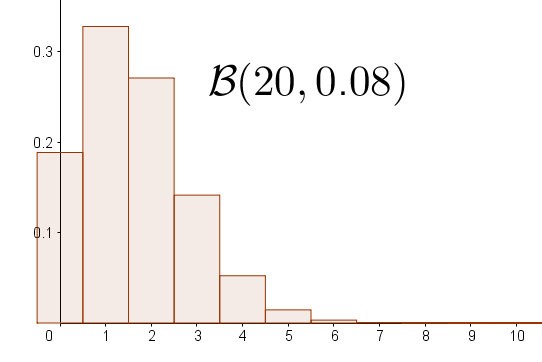
\includegraphics[width=0.22\textwidth]{img/binomiale1.png}
  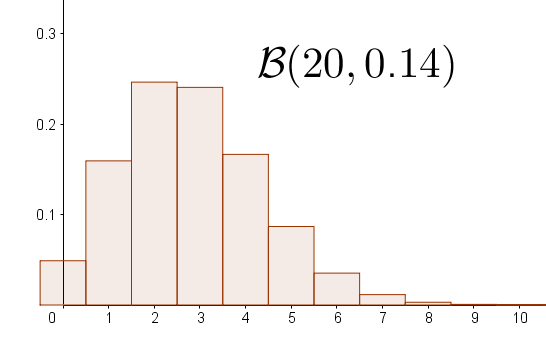
\includegraphics[width=0.22\textwidth]{img/binomiale2.png}
  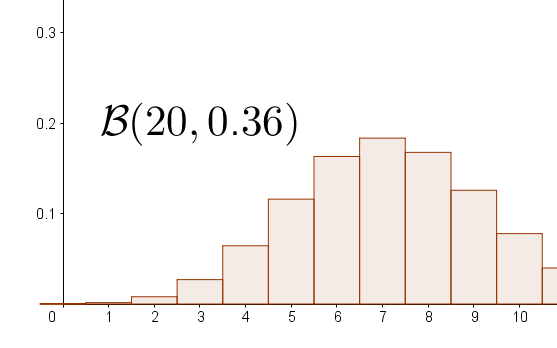
\includegraphics[width=0.22\textwidth]{img/binomiale3.png}
  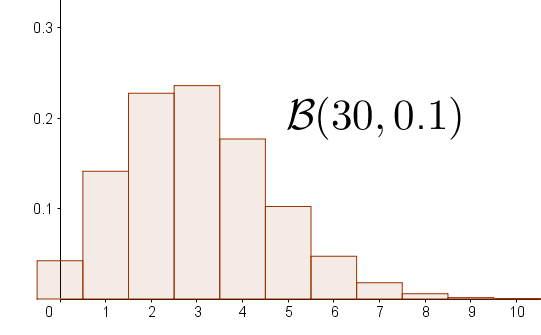
\includegraphics[width=0.22\textwidth]{img/binomiale4.png}
\end{center}

\begin{proprieta} Data una variabile discreta binomiale X di parametri $n$ e $p$, si dimostra che: 
\[\boxed{M(X) = n \,p} \qquad \boxed{V(X) = n \,p\,(1-p)}\]
\end{proprieta}

\begin{proof} Si usa la formula del binomio di Newton: \quad $\displaystyle (a+b)^N = \sum_{k=1}^N a^{n-k} b^k$
\end{proof}



\subsection{Distribuzione di Poisson}
L'ultima variabile che vediamo è la seguente:

\begin{definizione} Chiamiamo \emph{distribuzione di Poisson} $\mathcal{P}(\lambda)$ una variabile aleatoria discreta con parametro reale $\lambda >0$ tale che:
\[ x_k = k \in \mathbb{N} \qquad P(X=k)= \dfrac{\lambda^k}{k!} e^{-\lambda}\]
\end{definizione}

Viene usata per modellare il numero di eventi che avvengono in un certo periodo di tempo, quando è noto il numero medio di eventi che avvengono in quello stesso periodo di tempo. Il parametro $\lambda$ indica proprio quel numero medio di eventi.

\begin{osservazione} Notiamo che, al contrario della binomiale, la variabile di Poisson può assumere qualunque valore naturale (non è limitata!)
\end{osservazione}

\begin{esempio} Mediamente ad un call-center si ricevono 12 chiamate all'ora. Calcoliamo la probabilità di ricevere 1 sola chiamata in un'ora e la probabilità di ricevere tra le 8 e le 10 chiamate.
\[\begin{split}P(X=1) &= \dfrac{12^1}{1!} e^{-12} = 0,0000737 \approx 0 \\
P(8\leq X\leq 10) &= P(X = 8)+P(X=9)+P(X=10) = \dfrac{12^8}{8!} e^{-12} + \dfrac{12^9}{9!} e^{-12} + \dfrac{12^{10}}{10!} e^{-12} =\\
&= \dfrac{12^8}{8!} e^{-12} \tonda{1+\dfrac{12}{9}+\dfrac{12^2}{10\cdot 9}} \approx 25,77 \%\end{split}\]
\end{esempio}

\begin{esempio} Ogni ora partono, in media, 8 voli da un aeroporto cittadino. Qual'è la probabilità che,in 10 minuti, partano meno di 3 voli?\\[5pt]
Notiamo che, in questo caso, ci sono 2 tempi diversi, nel testo e nella domanda. Dobbiamo convertire la media dei voli in modo che combaci con quella richiesta dalla domanda.
\[\text{8 voli/ora} \quad \longrightarrow \quad \dfrac{\text{8 voli}}{\text{1 ora}}=\dfrac{\text{8 voli}}{\text{60 minuti}} = \dfrac{2}{15}\,\text{voli/minuto} \approx 0,13\,\text{voli/minuto}\]
Ora possiamo calcolare ciò che ci è stato richiesto:
\[\begin{split}P(X<3) &= P(X=0)+P(X=1)+P(X=2) = \dfrac{0,13^{0}}{0!} e^{-0,13}+\dfrac{0,13^{1}}{1!} e^{-0,13}+\dfrac{0,13^{2}}{2!} e^{-0,13}=\\
&= e^{-0,13} \tonda{1+0,13+\dfrac{0,13^2}{2}} \approx 99,97 \% \end{split}\]
\end{esempio}

\begin{proprieta} Data una variabile discreta di Poisson X di parametro $\lambda$, si dimostra che: 
\[\boxed{M(X) = \lambda} \qquad \boxed{V(X) = \lambda}\]
\end{proprieta}

\begin{osservazione} La distribuzione di Poisson viene usata come \emph{approssimazione della binomiale}, per valori molto grandi di $n$ e molto piccoli di $p$, utilizzando il parametro $\lambda = n\,p$
\end{osservazione}

\begin{esempio}
Una macchina produce pezzi difettosi con una media di 1 su 100. Qual'è la probabilità che, su 1000 pezzi, 30 siano difettosi?\\[5pt]
In questo caso si potrebbe usare una binomiale, in cui $n=1000$, $p=0,01$:
\[P(X=30) = \binom{1000}{30} \tonda{0,01}^{30} \tonda{1-0,01}^{970} \approx 1,42\cdot 10^{-7} \]
Usando l'approssimazione di Poisson invece, otteniamo ($\lambda=1000\cdot 0,01=10$):
\[P(X=30) = \dfrac{10^{30}}{30!} e^{-10} \approx 1,71\cdot 10^{-7} \]
\end{esempio}


\section{Variabili aleatorie continue}
\label{sec:continue}

\begin{definizione} Chiamiamo \emph{variabile aleatoria continua} una variabile aleatoria che può assumere qualunque valore $x \in \mathbb{R}$.
\end{definizione}

In questo caso la variabile aleatoria può essere vista come una funzione che associa ad ogni evento un numero reale $X:\Omega \longrightarrow \mathbb{R}\,, E \longmapsto X(E) $. Vediamo alcuni esempi:
\begin{itemize}
\item tempo di vita di una lampadina
\item prezzo di un titolo di mercato
\item  posizione di un granello di polvere in aria
\end{itemize}

Notiamo innanzitutto che non ha molto senso chiedersi quale sia la probabilità che X assuma un preciso valore. Avendo infinite possibilità, la probabilità che assuma esattamente quel valore scelto è nulla! Ha più senso chiedersi quale sia la probabilità che X assuma un valore preso all'interno di un dato intervallo.

\begin{definizione} Una funzione è detta \emph{densità di probabilità} se:
\[ \boxed{f(x) \geq 0 \quad \forall x \in \mathbb{R}} \qquad \boxed{ \int_{-\infty}^{+\infty} f(x)\, dx = 1}\]
\end{definizione}

In particolare, data una funzione densità di probabilità, rimane definita una variabile aleatoria X con la proprietà che:\\
\begin{minipage}[c]{.5\textwidth}
\[P(a \leq X \leq b) = \int_a^b f(x)\,dx \qquad \forall a,b \in \mathbb{R}\]
\end{minipage}
\begin{minipage}[c]{.5\textwidth}
\begin{center}
  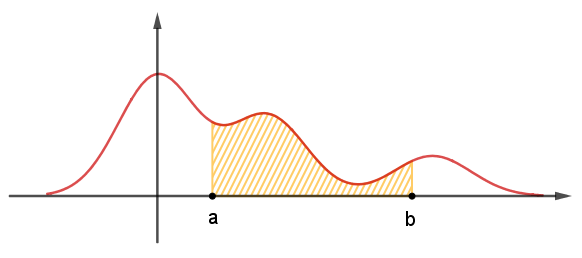
\includegraphics[width=0.8\textwidth]{img/Probabilita.png}
\end{center}
\end{minipage}


Le proprietà indicate nella definizione servono appunto a definire in modo coerente questa definizione. Infatti devono essere valide le proprietà base della probabilità:
\[P(\text{evento certo}) = 1 \qquad P(\text{evento impossibile}) = 0 \qquad P(\text{evento}) \in [0,1] \]

\begin{esempio}
Verifica che la funzione seguente rappresenta una densità di probabilità. In caso affermativo, calcola la probabilità che X sia compreso tra 0 e 1:\[f(x)= \dfrac{1}{\pi (1+x^2)} \qquad \longrightarrow \qquad \text{Notiamo subito che $f(x)>0 \quad\forall x \in \mathbb{R}$}\]
\[ \begin{split}\int_{-\infty}^{+\infty} f(x)\, dx &=\int_{-\infty}^{+\infty} \dfrac{1}{\pi (1+x^2)}\, dx = \dfrac{1}{\pi}\cdot \lim_{M \rightarrow +\infty} \int_{-M}^{+M} \dfrac{1}{ (1+x^2)}\, dx = \\[5pt]
&= \dfrac{1}{\pi}\cdot \lim_{M \rightarrow +\infty} \Big[\arctan{x}\Big]_{-M}^{+M} = \dfrac{1}{\pi} \Big[\arctan{\tonda{+\infty}}-\arctan{\tonda{-\infty}}\Big] = \dfrac{1}{\pi} \tonda{\dfrac{\pi}{2}+\dfrac{\pi}{2}} = 1 \end{split}\]
quindi si tratta veramente di una funzione densità di probabilità. Possiamo quindi calcolare:
\[P(0\leq X\leq 1)  = \int_0^1\dfrac{1}{\pi (1+x^2)}\, dx =  \dfrac{1}{\pi} \cdot \Big[\arctan{x}\Big]_{0}^1 = \dfrac{1}{\pi} \cdot \quadra{\dfrac{\pi}{4}-0} \approx 0,25 = 25 \%\]
\end{esempio}

\begin{definizione} Data una variabile aleatoria X con densità di probabilità $f(x)$ chiamiamo \emph{funzione di ripartizione} la funzione $F(x)$ definita da:
\[F(x) = P(X\leq x) = \int_{-\infty}^x f(t) \,dt\]
\end{definizione}
Si tratta, in altre parole, della funzione integrale di $f(x)$. Dalle regole del calcolo integrale ricaviamo immediatamente due proprietà:
\[a) \quad F'(x) = f(x) \quad \text{(F è la primitiva di f)} \hspace{1.5cm} b) \quad P(a \leq X \leq b) = F(b)-F(a)\]
\begin{minipage}[c]{.45\textwidth}
La seconda proprietà si può ricava in modo grafico anche visualizzando il disegno a lato: l'area del sottografico nell'intervallo $[a,b]$ si può calcolare come area in $[-\infty,b]$ meno area in $[-\infty,a]$
\end{minipage}
\begin{minipage}[c]{.55\textwidth}
\begin{center}
  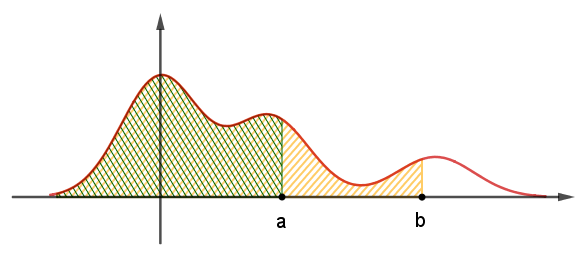
\includegraphics[width=0.9\textwidth]{img/FormulaAree.png}
\end{center}
\end{minipage}

\begin{esempio} Calcola la funzione di ripartizione di $f(x)=\dfrac{1}{\pi (1+x^2)}$ e calcola $P(0 \leq X \leq 1)$
\[F(x) = \int_{-\infty}^x f(t) \, dt = \dfrac{1}{\pi} \lim_{M \rightarrow +\infty} \Big[\arctan{t}\Big]_{-M}^x = \dfrac{1}{\pi} \tonda{\arctan{x}+\dfrac{\pi}{2}} =  \dfrac{1}{2}+\dfrac{1}{\pi} \arctan x\]
\[P(0\leq X \leq 1) = F(1)-F(0) = \tonda{\dfrac{1}{2}+\dfrac{1}{\pi} \arctan 1}-\tonda{\dfrac{1}{2}+\dfrac{1}{\pi} \arctan 0} = \dfrac{1}{4} = 0,25 = 25\%\]
\end{esempio}

\subsection{Valori sintetici delle distribuzioni continue}

Anche per le variabili aleatorie continue si definiscono media e varianza, in modo similare a quanto fatto per le variabili discrete:
\[\text{\textbf{Valor medio ($\mu$)}:}\quad  \boxed{M(X) = \int_{-\infty}^{+\infty} x \cdot f(x) \, dx}  \]
\[\text{\textbf{Varianza ($\sigma^2$)}:}\quad  \boxed{V(X) = \int_{-\infty}^{+\infty} (x- M(X))^2 \cdot f(x) \, dx}\]\\[4pt]
Si dimostra che valgono tutte le proprietà viste nel caso discreto. La dimostrazione si basa semplicemente sulle proprietà viste finora e sulle proprietà principali del calcolo integrale.

\begin{esempio} Calcola media e varianza della variabile aleatoria definita da $f(x) = \dfrac{1}{\pi (1+x^2)}$
\[\begin{split}M(X) &= \int_{-\infty}^{+\infty} x\cdot \dfrac{1}{\pi (1+x^2)} \, dx =  \dfrac{1}{\pi}\cdot  \lim_{M \rightarrow +\infty} \int_{-M}^{+M} \dfrac{x}{1+x^2} \,dx = \\
&= \dfrac{1}{\pi}\cdot  \lim_{M \rightarrow +\infty} \quadra{\dfrac{1}{2} \log \tonda{1+x^2}}_{-M}^{+M} =   \dfrac{1}{2 \pi}\cdot  \lim_{M \rightarrow +\infty} \quadra{\log \tonda{1+M^2}-\log \tonda{1+M^2}} =0\end{split}\]
\[\begin{split} V(X) &= \int_{-\infty}^{+\infty} \tonda{x-0}^2 \cdot \dfrac{1}{\pi (1+x^2)} \, dx =\dfrac{1}{\pi}\cdot \int_{-\infty}^{+\infty} \dfrac{x^2}{ 1+x^2} \, dx \\&=
=\dfrac{1}{\pi}\cdot  \lim_{M \rightarrow +\infty} \int_{-M}^{+M} \dfrac{x^2}{ 1+x^2} \, dx = \dfrac{1}{\pi}\cdot  \lim_{M \rightarrow +\infty} \int_{-M}^{+M} \dfrac{1+x^2-1}{ 1+x^2} \, dx = \\&=
\dfrac{1}{\pi}\cdot  \lim_{M \rightarrow +\infty} \quadra{\int_{-M}^{+M} \dfrac{1+x^2}{ 1+x^2}\, dx-\int_{-M}^{+M} \dfrac{1}{ 1+x^2}\, dx} = \\&=\dfrac{1}{\pi}\cdot  \lim_{M \rightarrow +\infty} \graffa{\Big[x\Big]_{-M}^{+M} - \Big[\arctan{x}\Big]_{-M}^{+M}} \\ &=   \dfrac{1}{\pi}\cdot  \lim_{M \rightarrow +\infty} \Big\{M-(-M)-\arctan{M}-\arctan{\tonda{-M}}\Big\} = +\infty \end{split}\]
\end{esempio}


\section{Distribuzioni continue di uso comune}
\label{sec:distrib_continue}

Anche per le variabili aleatorie continue, vediamo alcune tra le distribuzioni più utilizzate:

\subsection{Distribuzione uniforme}

\begin{definizione} Chiamiamo \emph{distribuzione continua uniforme} $\mathcal{U}([a,b])$ definita sull'intervallo $[a,b]$ la distribuzione di probabilità con densità data dalla funzione:
\[f(x) = \begin{cases} \dfrac{1}{b-a} & a\leq x\leq b \\
0 & \text{altrimenti}\end{cases}\]
\end{definizione}

\begin{minipage}[c]{.45\textwidth}
\'E facile verificare che $f(x)$ rappresenta veramente una densità di probabilità. Si potrebbe inoltre estendere la definizione a unione di più intervalli ed anche a casistiche più complesse.
\end{minipage}
\begin{minipage}[c]{.55\textwidth}
\begin{center}
  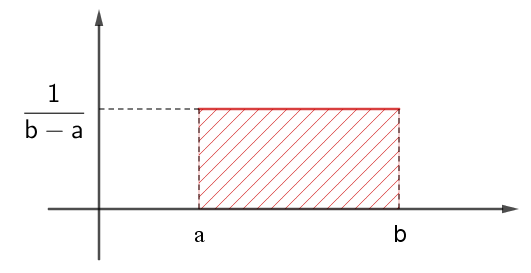
\includegraphics[width=0.9\textwidth]{img/Uniforme_continua.png}
\end{center}
\end{minipage}

\begin{esempio} Un fenomeno segue una distribuzione uniforme continua $\mathcal{U} ([-1,3])$. Calcola media, varianza e probabilità di ottenere un valore compreso tra 0 e 5.
\[\begin{split}M(X) &=  \int_{-\infty}^{+\infty} x\cdot f(x) \,dx = \underbrace{\cancel{\int_{-\infty}^{-1} x\cdot f(x) \,dx}}_{f(x)=0}+\underbrace{\int_{-1}^{3} x\cdot f(x) \,dx}_{f(x) = \frac{1}{4}}+ \underbrace{\cancel{\int_{3}^{+\infty} x\cdot f(x) \,dx}}_{f(x)=0} = \\ &=\int_{-1}^{3}  \frac{1}{4}\, x \,dx =\frac{1}{4} \cdot \Big[   x \Big]_{-1}^3 = \frac{1}{4}\cdot \Big[   3-(-1) \Big] = 1\\[6pt]
V(X) &=  \int_{-\infty}^{+\infty}\Big(x-1\Big)^2\cdot f(x) \,dx = \int_{-1}^{3}\Big(x-1\Big)^2\cdot \frac{1}{4} \,dx= \frac{1}{4} \Big[\frac{\tonda{x-1}^3}{3}\Big]_{-1}^3 = \frac{4}{3}  \\[6pt]
\end{split}\]
\[P(0\leq X \leq 5) =  \int_{0}^{5}  f(x) \,dx =  \underbrace{\int_{0}^{3} f(x) \,dx}_{f(x) = \frac{1}{4}}+ \underbrace{\cancel{\int_{3}^{5} f(x) \,dx}}_{f(x)=0} = \int_0^3 \frac{1}{4} \,dx = \frac{1}{4} \Big[x\Big]_0^3 = \frac{1}{4} \cdot 3 = \frac{3}{4}\]
\end{esempio}

\begin{proprieta} Data una variabile continua uniforme $\mathcal{U}([a,b])$, si dimostra che: 
\[\boxed{M(X) =\dfrac{a+b}{2}} \qquad \boxed{V(X) = \dfrac{(b-a)^2}{12}}\]
\end{proprieta}


\subsection{Distribuzione esponenziale}

\begin{definizione} Chiamiamo \emph{distribuzione continua esponenziale} $\mathcal{E}(\lambda)$ di parametro $\lambda$ la distribuzione di probabilità con densità data dalla funzione:
\[f(x) = \begin{cases} \lambda \, e^{-\lambda x} & x \geq 0 \\
0 & \text{altrimenti}\end{cases}\]
\end{definizione}

\begin{minipage}[c]{.45\textwidth}
Viene spesso utilizzata per modellare il tempo di vita di oggetti o fenomeni (infatti la probabilità che la vita di un oggetto abbia una durata molto grande è via via decrescente).
\end{minipage}
\begin{minipage}[c]{.55\textwidth}
\begin{center}
  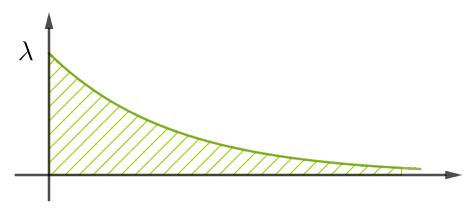
\includegraphics[width=0.9\textwidth]{img/Esponenziale.png}
\end{center}
\end{minipage}

\begin{esempio} Verifica che la funzione densità di $\mathcal{E} (5)$ rappresenta davvero una densità di probabilità continua. Dopo aver ricavato media e varianza, calcola la probabilità di ottenere un valore inferiore a 1.
\[\begin{split}\int_{-\infty}^{+\infty} f(x) \, dx &= \int_0^{+\infty} 5\, e^{-5x} \,dx  = \lim_{M\rightarrow +\infty} \int_0^M 5 \, e^{-5x} \,dx =  \lim_{M \rightarrow +\infty} \Big[-e^{-5x}\Big]_0^M = 1\end{split} \]
inoltre la funzione $f(x)$ è chiaramente positiva, quindi rappresenta una densità di probabilità.
\[\begin{split}M(X) &= \int_{-\infty}^{+\infty}x\cdot  f(x) \, dx =\int_{0}^{+\infty} 5x\, e^{-5x} \, dx =\lim_{M\rightarrow +\infty} \int_{0}^{M} \Big(-x\Big) \cdot \Big(-5\, e^{-5x}\Big) \\& = \text{(integrazione per parti)} = \lim_{M\rightarrow +\infty} \graffa{ \Big[-x \,e^{-5x}\Big]_0^M-\int_0^M -e^{-5x} \,dx} = \\
&=\lim_{M\rightarrow +\infty} \graffa{ \Big[-M \,e^{-5M}\Big]-\frac{1}{5}\Big[e^{-5x} \Big]_0^M} = \lim_{M\rightarrow +\infty} \graffa{-M \,e^{-5M}-\frac{1}{5} e^{-5M}+\frac{1}{5}} = \frac{1}{5} \end{split} \]
dove abbiamo usato il fatto che $\displaystyle \lim_{x\rightarrow +\infty} x e^{-x} = 0$ \;(si dimostra facilmente!). Per il calcolo della varianza possiamo usare invece la formula alternativa:
\[\begin{split}V(X) &= M(X^2)-M(X)^2 = \int_{-\infty}^{+\infty}x^2 \cdot  f(x) \, dx - \tonda{ \frac{1}{5}}^2 = \int_{0}^{+\infty}x^2 \cdot  5\,e^{-5x} \, dx -  \frac{1}{25} = \\ &= 
\lim_{M\rightarrow +\infty} \int_0^M \tonda{-x^2} \tonda{-5 e^{-5x}}\,dx  -  \frac{1}{25} =\\&= \lim_{M\rightarrow +\infty}\graffa{ \Big[ -x^2 e^{-5x} \Big]_0^M - \int_0^M -2x e^{-5x} \,dx}  -  \frac{1}{25}= \\
&=   \lim_{M\rightarrow +\infty}\Bigg\{-M^2 e^{-5M} +\frac{2}{5} \underbrace{\int_0^M 5x e^{-5x} \,dx}_{=M(X)}\Bigg\}  -  \frac{1}{25}= \frac{2}{25}-\frac{1}{25} = \frac{1}{25}
 \end{split} \]
\end{esempio}


\begin{proprieta} Data una variabile continua esponenziale $\mathcal{E}(\lambda)$, si dimostra che: 
\[\boxed{M(X) =\dfrac{1}{\lambda}} \qquad \boxed{V(X) = \dfrac{1}{\lambda^2}}\]
\end{proprieta}


\subsection{Distribuzione normale}

La più importante distribuzione (e la più usata)  è la distribuzione gaussiana, che prende il nome dal matematico tedesco Carl Friederich Gauss, forse il matematico più importante della storia, che analizzò e utilizzò questa distribuzione per studi astronomici.

\begin{definizione} Chiamiamo \emph{distribuzione normale} (o Gaussiana) $\mathcal{N}(\mu,\sigma^2)$ di parametri $\mu, \sigma^2 \in \mathbb{R}$ la distribuzione di probabilità con densità data dalla funzione:
\[f(x) =  \frac{1}{\sigma \sqrt{2 \pi}} e^{-\frac{(x-\mu)^2}{2 \sigma^2}}\]
\end{definizione}

\begin{minipage}[c]{.45\textwidth}
La distribuzione gaussiana viene utilizzata in moltissimi ambiti, come l'analisi degli errori, le scienze sociali, la statistica, \dots \\
Viene detta anche \textbf{campana di Gauss}, per la forma caratteristica.
\end{minipage}
\begin{minipage}[c]{.55\textwidth}
\begin{center}
  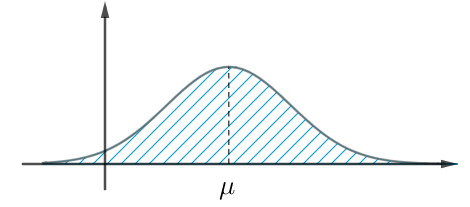
\includegraphics[width=0.9\textwidth]{img/Normale.png}
\end{center}
\end{minipage}

\begin{proprieta} Data una variabile normale $\mathcal{N}(\mu, \sigma^2)$, si dimostra che: 
\[\boxed{M(X) =\mu} \qquad \boxed{V(X) = \sigma^2}\]
\end{proprieta}

Nonostante il suo grande utilizzo nei più svariati ambiti disciplinari, questa distribuzione soffre di una problematica particolare: la funzione $f(x)$ infatti non ha una primitiva! Questo porta notevoli svantaggi di calcolo, ed è quindi necessario utilizzare delle tavole precompilate (dette \textbf{Tavole di Sheppard}) per il calcolo di probabilità che fanno uso di questa distribuzione. Le tavole riportano i valori dell'area sottesa alla distribuzione normale $\mathcal{N} (0,1)$ (detta \textbf{normale standard}) per cui, per calcolare i valori nel caso di una normale non standard è necessario usare il processo di \textbf{normalizzazione} visto in \ref{sec:02_standardizzate}.

\begin{esempio} Data una variabile aleatoria X che si distribuisce secondo una normale $\mathcal{N}(3,4)$, calcolare la probabilità che X sia compreso tra 0 e 6.\\[6pt]
Inizialmente normalizziamo la variabile: \(Z =\dfrac{X-\mu}{\sigma} = \dfrac{X-3}{2} \sim \mathcal{N}(0,1)\)
\[\begin{split}P(0\leq X \leq 6) &= P(0-3 \leq X-3 \leq 6-3) = P(-3 \leq X-3 \leq 3)=\\& = P\tonda{-\dfrac{3}{2}\leq \dfrac{X-3}{2} \leq \dfrac{3}{2}} = P\tonda{-\dfrac{3}{2}\leq Z \leq \dfrac{3}{2}} \end{split} \]
ma ora il calcolo si è ricondotto al calcolo dell'area del sottografico della distribuzione $\mathcal{N}(0,1)$, che è possibile ricavare dalle tavole di Sheppard. In realtà solitamente in queste tabelle viene indicata l'area in $(-\infty,k]$, quindi è necessario usare qualche trucchetto per terminare:
\[P\tonda{-\dfrac{3}{2}\leq Z \leq \dfrac{3}{2}} = P\tonda{Z \leq \dfrac{3}{2}}-P\tonda{Z \leq -\dfrac{3}{2}} \approx 0,9332-0,0668=0,8664 = 86,64 \%\]
\end{esempio}
